Nachdem wir uns in dieser Arbeit damit beschäftigt haben, wie \ac{qc} die aktuelle asymmetrische Kryptographie brechen kann und wie mit diesem Problem auf einer technischen Ebene umgegangen wird, gilt es noch eine weitere Frage zu beantworten: \\
\textit{Warum müssen wir uns schon jetzt mit dieser potentiellen Gefahr auseinandersetzen?}\\
Ein Großteil der vorgestellen Konzepte und Algorithmen sind nur theoretischer Natur und aktuelle \ac{qc} sind nicht in der Lage zum Beispiel RSA zu decodieren. Warum also hat das \ac{nist} seine Ausschreibung für einen quantensicheren Algorithmus gestartet? Warum sollte die Gefahr eines \ac{qc}s auf die Kryptographie schon jetzt ernst genommen werden?\\
Zum einen gilt es die Frage zu beantworten, wann es wahrscheinlich ist, dass ein \ac{qc} in der Lage sein wird eine mit RSA-2048 Bit verschlüsselte Nachricht zu entschlüsseln. Das theoretische Minimum an benötigten Qubits hierfür liegt laut Abschätzungen der Schweizer IT-Sicherheitsfirma \textit{Kudelski Security} bei 6190 logischen Qubits \cite{gagliardoni_quantum_2021}. Dies berücksichtigt jedoch nicht Faktoren wie Implementierungs-Details und Fehlerkorrektur. Einer anderen Schätzung zufolge, würden eher um die 10.000 reale Qubits benötigt werden \cite{ziegler_online_2015}. Wie Lange wird es dauern bis ein \ac{qc} mit einer solchen Anzahl an Qubits Realität ist?\\
Schaut man auf die \textit{Timeline} der Firma IBM (siehe Grafik \ref{fig:ibm-rm}) so sieht man, dass der aktuelle Entwicklungsstand ein \ac{qc} mit 433 Qubits ist. Dies stellt schon ein enormes Wachstum zu den 27 Qubits in 2019 dar. Der Plan ist es bis 2025 auf ungefähr 4000 Qubits zu gelangen und nach 2026 10.000 und mehr Qubits anzustreben \cite{noauthor_ibm_2015}.\\
Diese Vorhersage deckt sich auch mit den Ansichten führender Experten in dem Gebiet der Quantenkryptographie. Die Ergebnisse einer Befragung des \textit{Global Risk Institutes} an der 47 Forschende teilnahmen, sind in der Abbildung \ref{fig:qx-approx} veranschaulicht. Es wird für sehr wahrscheinlich gehalten, dass in den nächsten 15 bis 20 Jahren ein \ac{qc} in der Lage sein wird RSA-2048 zu brechen. Mindestens aber in 30 Jahren soll dies mit nahezu vollständiger Sicherheit möglich sein \cite{noauthor_2021_nodate}.

\begin{figure}[!hbt]
    \centering
    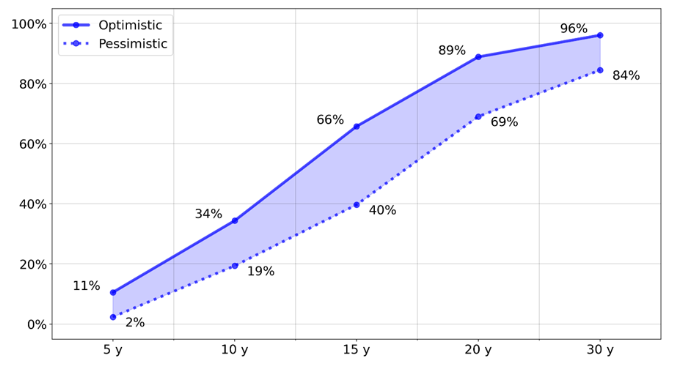
\includegraphics[width=0.5\textwidth]{images/estiamte-qc.png}
    \caption{Wahrscheinlichkeit wann laut Experten des Quantencomputing RSA-2048 durch einen \ac{qc} gebrochen sein kann \cite{noauthor_2021_nodate}}
    \label{fig:qx-approx}
\end{figure}\